\documentclass[hidelinks, 11pt, fleqn]{article}   	% use "amsart" instead of "article" for AMSLaTeX format
\usepackage{geometry}                		% See geometry.pdf to learn the layout options. There are lots.
\usepackage{tikz}
\usepackage{listings}
\usepackage{color}



\renewcommand{\lstlistingname}{Algorithm}% Listing -> Algorithm

\lstdefinestyle{mystyle}{
	backgroundcolor=\color{backcolour},   
	commentstyle=\color{codegray},
	keywordstyle=\color{red},
	numberstyle=\tiny\color{lightgray},
	stringstyle=\color{codepurple},
	basicstyle=\footnotesize,
	breakatwhitespace=false,         
	breaklines=true,                 
	captionpos=b,                    
	keepspaces=true,                 
	numbers=left,                    
	numbersep=5pt,                  
	showspaces=false,                
	showstringspaces=false,
	showtabs=false,                  
	tabsize=4
}

\lstset{style=mystyle}

\usepackage{amsmath}
\usepackage{mathtools}
\usepackage{algorithm}
\usepackage{algpseudocode}
\geometry{letterpaper}                   		% ... or a4paper or a5paper or ... 
%\geometry{landscape}                		% Activate for rotated page geometry
%\usepackage[parfill]{parskip}    		% Activate to begin paragraphs with an empty line rather than an indent
\usepackage{graphicx}				% Use pdf, png, jpg, or eps§ with pdflatex; use eps in DVI mode
\usepackage{subcaption}
\usepackage{hyperref}
% TeX will automatically convert eps --> pdf in pdflatex		
\usepackage{amssymb}

%SetFonts

%SetFonts
\newtagform{brackets}{[}{]}
\usetagform{brackets}

\title{\textbf{G-Code Implementation}}
\author{Patrick Sorn}
%\date{}							% Activate to display a given date or no date

\begin{document}
\maketitle
\tableofcontents 
\pagebreak
\section{G00 - Rapid Positioning}
Rapid positioning mode does not care which axis movement completes first, it just let's the stepper motors run at max speed till they reach their destination.
\begin{figure}[h]
	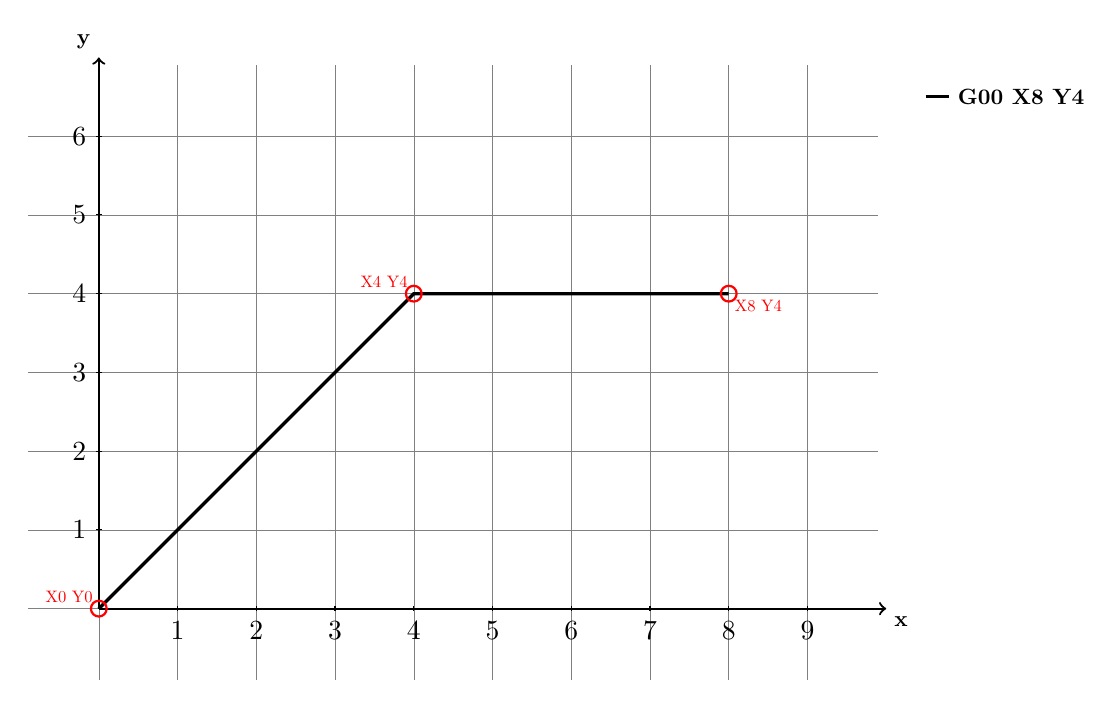
\begin{tikzpicture}
	% draw coordinate system
	\draw[step=1cm,gray,very thin] (-0.9,-0.9) grid (9.9,6.9);
	\draw[->,thick] (0,0) -- (10,0) node[anchor=north west,scale=0.8] {\textbf{x}};
	\draw[->,thick] (0,0) -- (0,7) node[anchor=south east,scale=0.8] {\textbf{y}};
	% axis labels
	\foreach \x in {1,2,3,4,5,6,7,8,9}
		\draw (\x cm,1pt) -- (\x cm,-1pt) node[anchor=north] {$\x$};
	\foreach \y in {1,2,3,4,5,6}
		\draw (1pt,\y cm) -- (-1pt,\y cm) node[anchor=east] {$\y$};
	% draw movement
	\draw[very thick] (0,0) -- (4,4) -- (8,4);
	\draw[red, thick] (0,0) circle (0.1cm);
	\draw[red, thick] (0,0) node[anchor=south east, scale=0.6] {X0 Y0};
	\draw[red, thick] (4,4) circle (0.1cm);
	\draw[red, thick] (4,4) node[anchor=south east, scale=0.6] {X4 Y4};
	\draw[red, thick] (8,4) circle (0.1cm);
	\draw[red, thick] (8,4) node[anchor=north west, scale=0.6] {X8 Y4};
	% draw legend
	\draw[very thick] (10.5,6.5) -- (10.8,6.5) node[anchor=west,scale=0.8] {\textbf{G00 X8 Y4}};
	\end{tikzpicture}
	\caption{Rapid positioning in detail (G00).}
	\label{fig:g00_detail}
\end{figure}
\pagebreak
\section{G01 - Linear Interpolation}
Linear interpolation is required to make coordinated movements across axis. Therefore we have to synchronize axis movement in order to have all involved axes reach destination at the same time point. X and Y represent step counts of two independent axis movements. The zig-zag-pattern tries to approximate the ideal movement.
\subsection{Function}
\begin{figure}[h]
	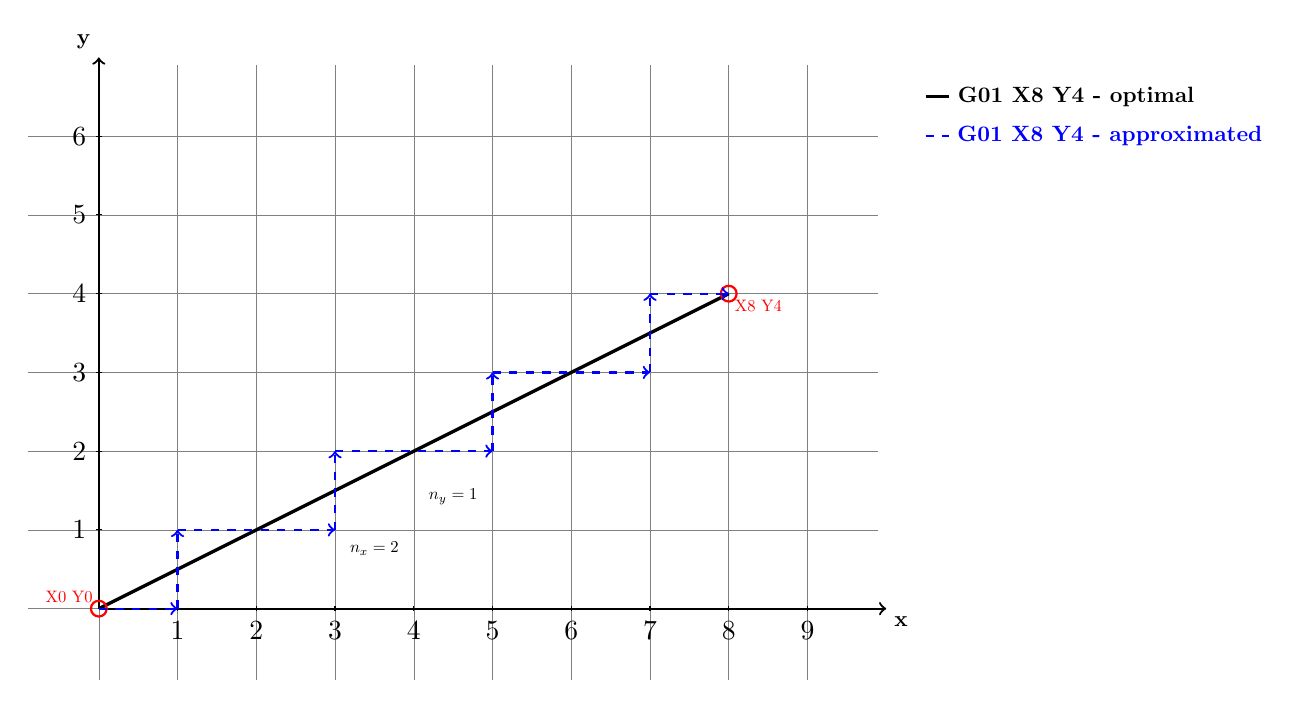
\begin{tikzpicture}
	% draw coordinate system
	\draw[step=1cm,gray,very thin] (-0.9,-0.9) grid (9.9,6.9);
	\draw[->,thick] (0,0) -- (10,0) node[anchor=north west,scale=0.8] {\textbf{x}};
	\draw[->,thick] (0,0) -- (0,7) node[anchor=south east,scale=0.8] {\textbf{y}};
	% axis labels
	\foreach \x in {1,2,3,4,5,6,7,8,9}
		\draw (\x cm,1pt) -- (\x cm,-1pt) node[anchor=north] {$\x$};
	\foreach \y in {1,2,3,4,5,6}
		\draw (1pt,\y cm) -- (-1pt,\y cm) node[anchor=east] {$\y$};
	% draw movement
	\draw[very thick] (0,0) -- (8,4);
	\draw[red, thick] (0,0) circle (0.1cm);
	\draw[red, thick] (0,0) node[anchor=south east, scale=0.6] {X0 Y0};
	\draw[red, thick] (8,4) circle (0.1cm);
	\draw[red, thick] (8,4) node[anchor=north west, scale=0.6] {X8 Y4};
	% draw steps
	\draw[blue,thick,dashed,->] (0,0) -- (1,0);
	\draw[blue,thick,dashed,->] (1,0) -- (1,1);
	\draw[blue,thick,dashed,->] (1,1) -- (3,1);
	\draw[blue,thick,dashed,->] (3,1) -- (3,2);
	\draw[blue,thick,dashed,->] (3,2) -- (5,2);
	\draw[blue,thick,dashed,->] (5,2) -- (5,3);
	\draw[blue,thick,dashed,->] (5,3) -- (7,3);
	\draw[blue,thick,dashed,->] (7,3) -- (7,4);
	\draw[blue,thick,dashed,->] (7,4) -- (8,4);
	\draw[thick] (3.5,0.6) node[anchor=south, scale=0.6] {$n_x=2$};
	\draw[thick] (4.5,1.6) node[anchor=north, scale=0.6] {$n_y=1$};
	% draw legend
	\draw[very thick] (10.5,6.5) -- (10.8,6.5) node[anchor=west,scale=0.8] {\textbf{G01 X8 Y4 - optimal}};
	\draw[blue,thick,dashed] (10.5,6) -- (10.8,6) node[anchor=west,scale=0.8] {\textbf{G01 X8 Y4 - approximated}};
	\end{tikzpicture}
	\caption{Linear interpolation in detail (G01).}
	\label{fig:g01_detail}
\end{figure}
\subsection{Algorithm}
\begin{algorithm}
	\caption{Calculate interpolation}
	\begin{algorithmic}[1]
		\State $x_c \gets 0$
		\State $y_c \gets 0$
		\If{$x > $y}
			\State $x_s \gets x / y$
			\State $y_s \gets 1$
			\State $i \gets 0$
			\While{$i < y$}
				\State $x_c \gets round(x_c + x_s)$
				\State $y_c \gets y_c + y_s$
				\State $i \gets i + 1$
			\EndWhile
		
		\Else
			\State $x_s \gets 1$
			\State $y_s \gets y / x$
			\State $i \gets 0$
			\While{$i < x$}
				\State $x_c \gets x_c + x_s$
				\State $y_c \gets round(y_c + y_s)$
				\State $i \gets i + 1$
			\EndWhile
		\EndIf
	\end{algorithmic}
\end{algorithm}
\pagebreak
\section{G02 - Circular Interpolation (clockwise)}
Circular interpolation is required to draw round corners and cut circle with bigger radius out of the material. To do so, we have to use the midpoint circle algorithm and follow the path with steps. However this movement is much more complicated as we have also given axis cutoff values, which influence the starting angle of our movement.
\subsection{The Parameter I}
The parameter I regulates the X-axis cutoff for the circular movement.
\begin{figure}[h]
	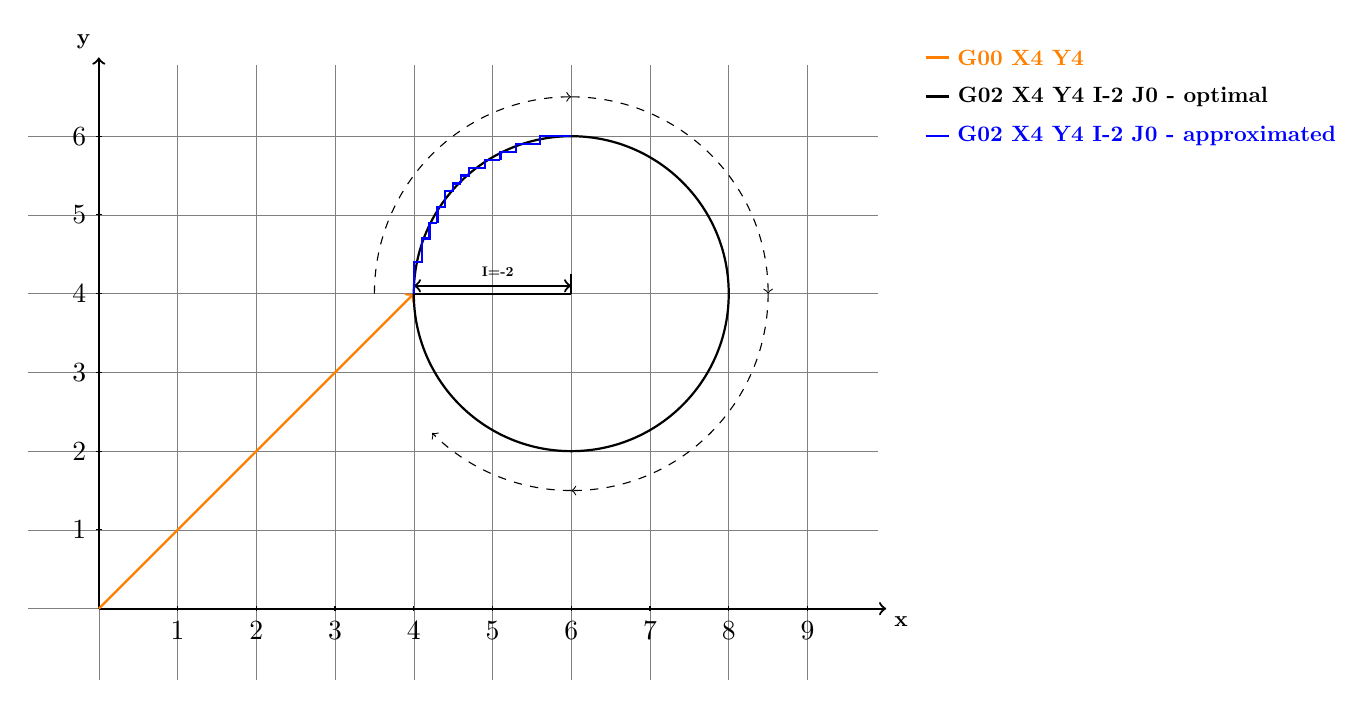
\begin{tikzpicture}
	% draw coordinate system
	\draw[step=1cm,gray,very thin] (-0.9,-0.9) grid (9.9,6.9);
	\draw[->,thick] (0,0) -- (10,0) node[anchor=north west,scale=0.8] {\textbf{x}};
	\draw[->,thick] (0,0) -- (0,7) node[anchor=south east,scale=0.8] {\textbf{y}};
	% axis labels
	\foreach \x in {1,2,3,4,5,6,7,8,9}
		\draw (\x cm,1pt) -- (\x cm,-1pt) node[anchor=north] {$\x$};
	\foreach \y in {1,2,3,4,5,6}
		\draw (1pt,\y cm) -- (-1pt,\y cm) node[anchor=east] {$\y$};
	% draw movement	
	\draw[orange,thick,->] (0,0) -- (4,4);
	\draw[thick] (6,4) circle (2);
	\draw[dashed,->] (3.5,4) arc (-180:-270:2.5);
	\draw[dashed,->] (6,6.5) arc (-270:-360:2.5);
	\draw[dashed,->] (8.5,4) arc (0:-90:2.5);
	\draw[dashed,->] (6,1.5) arc (-90:-135:2.5);
	%\draw[red, thick] (3,4.5) circle (0.1cm);
	%\draw[red, thick] (3,4.5) node[anchor=south east, scale=0.6] {Start/End Point - X4 Y4};
	%\draw[red,dashed,->] (3,4.5) -- (4,4);
	%\draw[thick,dashed,->] (4,4) -- (4,5);
	\draw[thick] (4,4) -- (6,4);
	\draw[thick,<->] (4,4.1) -- (6,4.1);
	\draw[thick] (6,4) -- (6,4.25);
	\draw[thick] (4.8,4.15) node[anchor=south west,scale=0.5] {\textbf{I=-2}};
	%draw steps
	\draw[blue,thick] (4.0,4.0) -- (4.0,4.4) -- (4.1,4.4) -- (4.1,4.7) -- (4.2,4.7) -- (4.2,4.9) -- (4.3,4.9);
	\draw[blue,thick] (4.3,4.9) -- (4.3,5.1) -- (4.4,5.1) -- (4.4,5.3) -- (4.5,5.3) -- (4.5,5.4) -- (4.6,5.4);
	\draw[blue,thick] (4.6,5.4) -- (4.6,5.5) -- (4.7,5.5) -- (4.7,5.6) -- (4.9,5.6) -- (4.9,5.7) -- (5.1,5.7);
	\draw[blue,thick] (5.1,5.7) -- (5.1,5.8) -- (5.3,5.8) -- (5.3,5.9) -- (5.6,5.9) -- (5.6,6.0) -- (6.0,6.0);
	% draw legend
	\draw[orange,thick] (10.5,7) -- (10.8,7) node[anchor=west,scale=0.8] {\textbf{G00 X4 Y4}};
	\draw[very thick] (10.5,6.5) -- (10.8,6.5) node[anchor=west,scale=0.8] {\textbf{G02 X4 Y4 I-2 J0 - optimal}};
	\draw[blue,thick] (10.5,6) -- (10.8,6) node[anchor=west,scale=0.8] {\textbf{G02 X4 Y4 I-2 J0 - approximated}};
	\end{tikzpicture}
	\caption{Circular interpolation in detail (G02, Parameter I).}
	\label{fig:g02i_detail}
\end{figure}
\pagebreak
\subsection{The Parameter J}
The parameter J regulates the Y-axis cutoff for the circular movement.
\begin{figure}[h]
	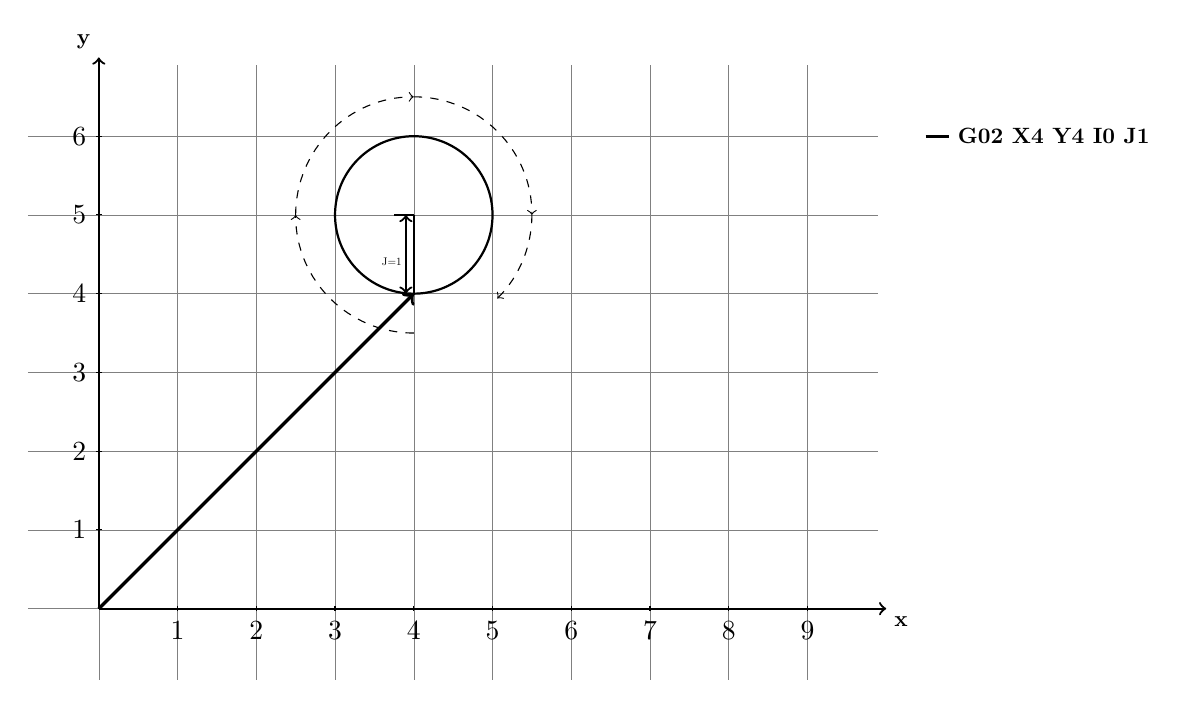
\begin{tikzpicture}
	% draw coordinate system
	\draw[step=1cm,gray,very thin] (-0.9,-0.9) grid (9.9,6.9);
	\draw[->,thick] (0,0) -- (10,0) node[anchor=north west,scale=0.8] {\textbf{x}};
	\draw[->,thick] (0,0) -- (0,7) node[anchor=south east,scale=0.8] {\textbf{y}};
	% axis labels
	\foreach \x in {1,2,3,4,5,6,7,8,9}
	\draw (\x cm,1pt) -- (\x cm,-1pt) node[anchor=north] {$\x$};
	\foreach \y in {1,2,3,4,5,6}
	\draw (1pt,\y cm) -- (-1pt,\y cm) node[anchor=east] {$\y$};
	% draw movement	
	\draw[very thick,->] (0,0) -- (4,4);
	\draw[thick] (4,5) circle (1);
	\draw[dashed,->] (4,3.5) arc (-90:-180:1.5);
	\draw[dashed,->] (2.5,5) arc (-180:-270:1.5);
	\draw[dashed,->] (4,6.5) arc (-270:-360:1.5);
	\draw[dashed,->] (5.5,5) arc (0:-45:1.5);
	%\draw[blue,dashed,->] (5.5,5) arc (0:-90:1.5);
	\draw[thick] (4,4) -- (4,5);
	\draw[thick,<->] (3.9,4) -- (3.9,5);
	\draw[thick] (3.75,5) -- (4,5);
	\draw[thick] (3.9,4.4) node[anchor=east,scale=0.4] {J=1};
	% draw legend
	\draw[very thick] (10.5,6) -- (10.8,6) node[anchor=west,scale=0.8] {\textbf{G02 X4 Y4 I0 J1}};
	\end{tikzpicture}
	\caption{Circular interpolation in detail (G02, Parameter J).}
	\label{fig:g02j_detail}
\end{figure}
\pagebreak
\subsection{The Parameter R}
The parameter R regulates the X-axis cutoff for the circular movement.
\begin{figure}[h]
	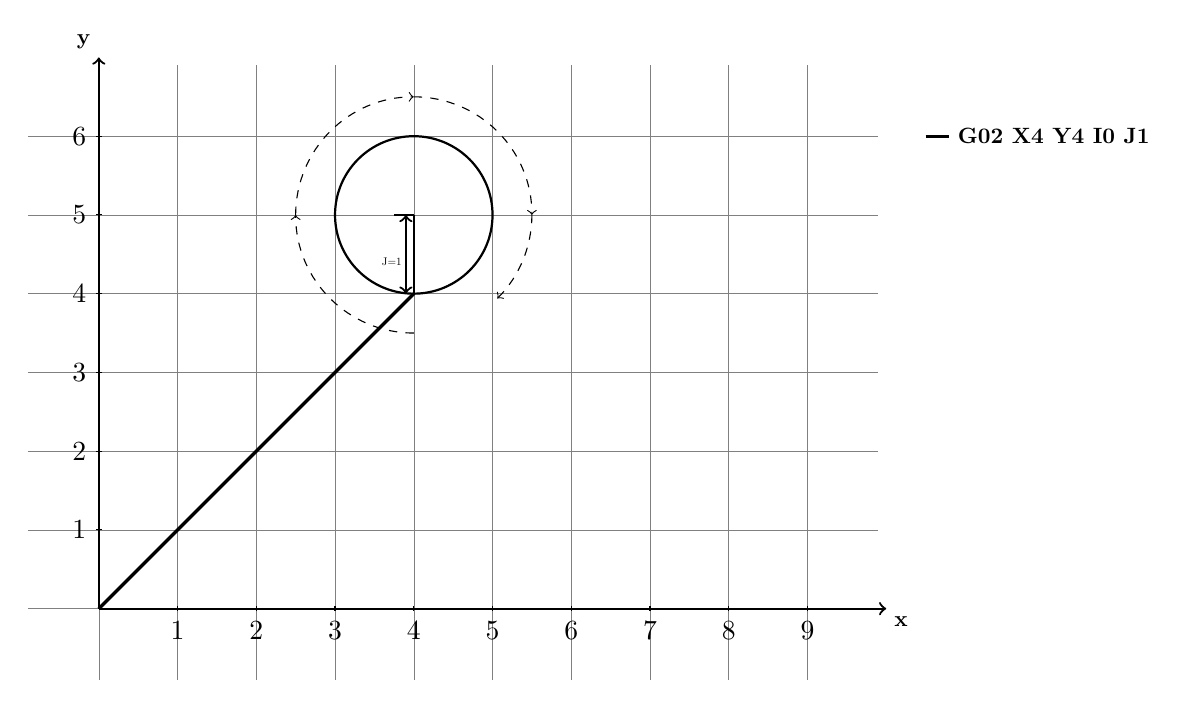
\begin{tikzpicture}
	% draw coordinate system
	\draw[step=1cm,gray,very thin] (-0.9,-0.9) grid (9.9,6.9);
	\draw[->,thick] (0,0) -- (10,0) node[anchor=north west,scale=0.8] {\textbf{x}};
	\draw[->,thick] (0,0) -- (0,7) node[anchor=south east,scale=0.8] {\textbf{y}};
	% axis labels
	\foreach \x in {1,2,3,4,5,6,7,8,9}
	\draw (\x cm,1pt) -- (\x cm,-1pt) node[anchor=north] {$\x$};
	\foreach \y in {1,2,3,4,5,6}
	\draw (1pt,\y cm) -- (-1pt,\y cm) node[anchor=east] {$\y$};
	% draw movement	
	\draw[very thick] (0,0) -- (4,4);
	\draw[thick] (4,5) circle (1);
	\draw[dashed,->] (4,3.5) arc (-90:-180:1.5);
	\draw[dashed,->] (2.5,5) arc (-180:-270:1.5);
	\draw[dashed,->] (4,6.5) arc (-270:-360:1.5);
	\draw[dashed,->] (5.5,5) arc (0:-45:1.5);
	%\draw[blue,dashed,->] (5.5,5) arc (0:-90:1.5);
	\draw[thick] (4,4) -- (4,5);
	\draw[thick,<->] (3.9,4) -- (3.9,5);
	\draw[thick] (3.75,5) -- (4,5);
	\draw[thick] (3.9,4.4) node[anchor=east,scale=0.4] {J=1};
	% draw legend
	\draw[very thick] (10.5,6) -- (10.8,6) node[anchor=west,scale=0.8] {\textbf{G02 X4 Y4 I0 J1}};
	\end{tikzpicture}
	\caption{Circular interpolation in detail (G02, Parameter R).}
	\label{fig:g02r_detail}
\end{figure}
\pagebreak
\section{G03 - Circular Interpolation (counterclockwise)}
\end{document}